\chapter{مفاهیم پایه}
در این فصل به معرفی مفاهیم پایه موردنیاز برای درک قسمت‌های مختلف پروژه و جزییات پیاده‌سازی آن پرداخته می‌شود.

\newcommand{\dd}[1]{\mathrm{d}#1}

% Quantum Computation

\section{محاسبات کوانتومی}

\subsection{سیستم‌های تک‌کیوبیتی}

طبق قوانین فیزیک کوانتومی، حالت یک سیستم می‌تواند به صورت ترکیب خطی‌ای از چند حالت پایه باشد، که این حالت‌های پایه، حالت‌هایی هستند که در قوانین فیزیک کلاسیک نیز حالات صحیحی برای توصیف سیستم هستند.
در محاسبات کوانتومی از بردارهای عمودی برای نشان‌دادن وضعیت یک سیستم استفاده می‌شود و وضعیت سیستم‌های چندکیوبیتی را نیز می‌توان از روی بردارهای یک سیستم تک‌کیوبیتی نیز ساخت.
\\
به طور معمول، در محاسبات کوانتومی، صرفا سیستم‌هایی که دارای تنها دو حالت پایه هستند بررسی می‌شوند، به همین علت، بردارهای فضای حالات سیستم‌های تک‌کیوبیتی ۲-بعدی هستند. لذا دو بردار مستقل یکه به عنوان بردارهای پایه‌ی این فضا تعیین داده می‌شوند که رابطه‌ی ۱-به-۱ ای با حالات پایه‌ی بیت‌های کلاسیک دارند.
این حالات پایه به صورت زیر تعیین می‌شوند:
\begin{equation}
    |0\rangle = \begin{bmatrix} 1 \\ 0 \end{bmatrix} 
    \mspace{18mu}
    |1\rangle = \begin{bmatrix} 0 \\ 1 \end{bmatrix}
\end{equation} 
\myequations{بردارهای پایه تک‌کیوبیتی}

نشان دادن بردارهای حالت به صورت 
\lr{$|0\rangle$} و \lr{$|1\rangle$}
به نمادگذاری \lr{bra-ket} دیراک
\fnote{Dirac's bra-ket notation}
معروف است و به ازای هر
\lr{ket}
به صورت زیر:
\begin{equation}
    |\psi\rangle = \alpha |0\rangle + \beta |1\rangle
    = \begin{bmatrix}
    \alpha \\[3pt]
    \beta
    \end{bmatrix}
\end{equation}
یک \lr{bra}
به این صورت تعریف می‌شود:
\begin{equation}
    \langle \psi| = \alpha^* \langle0| + \beta^* \langle1| = \begin{bmatrix} \alpha^* & \beta^* \end{bmatrix} 
\end{equation}

که در این‌جا نماد \lr{$\alpha^*$}
به معنای مزدوج مخلط 
\fnote{Complex conjugate}
عدد \lr{$\alpha$}
است.
\newpage

حالت‌های سیستم در فیزیک کوانتومی در اکثر اوقات به صورت بردارهای مختلط بهنجار
\fnote{Normalizable}
نشان داده می‌شوند.
\begin{equation}
    |\psi\rangle = \alpha |0\rangle + \beta |1\rangle = \begin{bmatrix} \alpha \\ \beta \end{bmatrix} 
    ; \mspace{18mu}
    \alpha, \beta \in \mathbb{C}
\end{equation}
% \newpage
\myequations{فرم کلی بردار وضعیت سیستم تک کیوبیتی}
که به امر ایجاد یک بردار وضعیت از ترکیب خطی دو بردار وضعیت دیگر، اصل برهم‌نهی کوانتومی
\fnote{Quantum Superposition}
گفته می‌شود.

بهنجار بودن به معنای صدق شرایط زیر است:
\begin{equation}
    \alpha\alpha^* + \beta\beta^* = |\alpha|^2 + |\beta|^2 = 1
\end{equation}
\myequations{شرط بهنجار بودن}
% \newpage
\begin{figure}
	\centering
	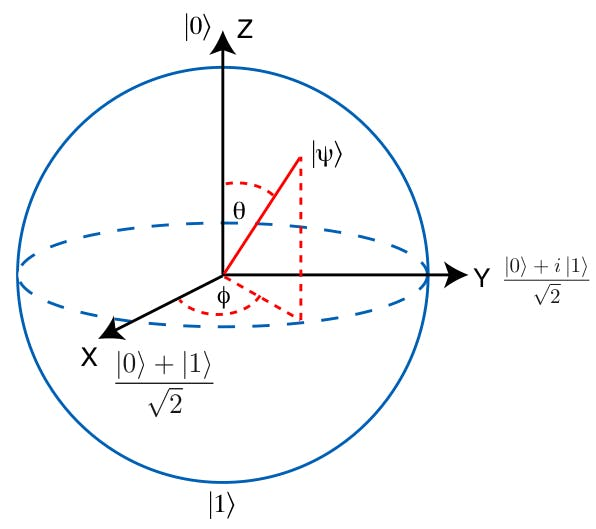
\includegraphics[scale=0.4]{figures/bloch.jpg}
	\caption{کره‌ی بلاخ}
	\label{fig:bloch}
\end{figure}
به علت شرط بهنجاری، می‌توان حالت کلی یک سیستم تک‌کیوبیتی را به صورت زیر نیز نوشت:
\begin{equation}
|\psi\rangle = \begin{bmatrix} e^{i\phi_1}\cos{\tfrac{\theta}{2}} \\[6pt] e^{i\phi_2}\sin{\tfrac{\theta}{2}} \end{bmatrix} 
\mspace{18mu}
\theta, \phi_1, \phi_2 \in {\rm I\!R}
\end{equation}
\myequations{حالت معادل فرم کلی بردار تک‌کیوبیتی}

که آن را می‌توان به صورت زیر نیز نوشت:
\begin{equation}
|\psi\rangle = e^{i\phi_1} \begin{bmatrix} \cos{\tfrac{\theta}{2}} \\[6pt] e^{i\phi_2-\phi_1}\sin{\tfrac{\theta}{2}} \end{bmatrix} = e^{i\phi_1} \begin{bmatrix} \cos{\tfrac{\theta}{2}} \\[6pt] e^{i\phi}\sin{\tfrac{\theta}{2}} \end{bmatrix}
\Rightarrow |\psi\rangle = \begin{bmatrix} \cos{\tfrac{\theta}{2}} \\[6pt] e^{i\phi}\sin{\tfrac{\theta}{2}} \end{bmatrix}
\end{equation}
\myequations{مهم نبودن فاز کلی سیستم}
در این معادله،
\lr{$\phi_1$}
 فاز کلی سیستم نامیده می‌شود که طبق قوانین فیزیک کوانتومی، در رفتار سیستم فاقد اهمیت است و به همین علت در مرحله‌ی آخر از آن صرف نظر شده‌است. \\
در نهایت، حالت کلی یک کیوبیت را می‌توان با استفاده از ابزاری به نام کره‌ی بلاخ (شکل
\ref{fig:bloch})
نمایش داد.

\subsection{سیستم‌های چندکیوبیتی}
دو سیستم تک‌کیوبیتی جداگانه را می‌توان به طور مجزا و به صورت زیر نمایش داد:
\begin{equation}
|a\rangle = \begin{bmatrix} a_0 \\ a_1 \end{bmatrix}, \quad |b\rangle = \begin{bmatrix} b_0 \\ b_1 \end{bmatrix}
\end{equation}
\myequations{دو کیوبیت مجزا}
در عین حال، می‌توانیم بردار وضعیت آن‌ها را به صورت هم‌زمان با استفاده از عملگری به نام ضرب تانسوری
\fnote{Tensor product}
تعریف کنیم که به صورت زیر عمل می‌کند:
\begin{equation}
|b\rangle \otimes |a\rangle = \begin{bmatrix} b_0 \times \begin{bmatrix} a_0 \\ a_1 \end{bmatrix} \\[12pt] b_1 \times \begin{bmatrix} a_0 \\ a_1 \end{bmatrix} \end{bmatrix} = \begin{bmatrix} b_0 a_0 \\[2pt] b_0 a_1 \\[2pt] b_1 a_0 \\[2pt] b_1 a_1 \end{bmatrix} = |ba\rangle
\end{equation}
\myequations{ضرب تانسوری}

\subsection{درهم‌تنیدگی}

درهم‌تنیدگی کوانتومی\fnote{Quantum Entanglement}
، یکی از اصول فیزیک کوانتومی است و به این معناست که برخی بردار وضعیت‌های سیستم‌های چندکیوبیتی را نمی‌توان به صورت ضرب تانسوری دو بردار تک‌کیوبیتی مجزا تعریف کرد. این امر نشان‌گر این است که وضعیت این دو کیوبیت به هم وابسته هستند.
به عنوان مثال، اگر بردارهای زیر که در محاسبات کوانتومی به وضعیت‌های بل 
\fnote{Bell states}
معروف هستند را در نظر بگیریم:
\begin{equation}
|{\Phi_\pm}\rangle = \frac{1}{\sqrt 2}\big(|0\rangle| 0\rangle\pm |1\rangle| 1\rangle\big), \qquad |{\Psi_{\pm}}\rangle=\frac{1}{\sqrt 2}\big(|0\rangle| 1\rangle\pm  |1\rangle|0\rangle\big)
\end{equation}
\myequations{بردار وضعیت‌های بل}

مشاهده می‌کنیم که هیچ‌کدام از این بردارها را نمی‌توان به صورت ضرب تانسوری‌ای از ترکیب خطی بردارهای
\lr{$|0\rangle$} و \lr{$|1\rangle$}
نوشت.

\subsection{گیت‌های کوانتومی}
در کامپیوترهای کلاسیک، محاسبات با استفاده از گیت‌هایی همانند 
\lr{AND}، \lr{OR} و NOT
انجام می‌شود.
معادل این گیت‌ها در محاسبات کوانتومی، گیت‌های کوانتومی هستند. این گیت‌ها به فرم ماتریس‌های یکانی 
\fnote{Unitary matrix}
\lr{$2^n \times 2^n$}
هستند که در این‌جا، عدد \lr{$n$}
نشان‌گر تعداد کیوبیت‌های سیستم است.

\subsubsection{
    گیت‌های کوانتومی تک‌کیوبیتی
}
در این بخش، صرفا تعدادی از گیت‌های کوانتومی به صورت خلاصه معرفی می‌شوند و اثر آن‌ها بر روی پایه‌های برداری فضای سیستم‌های تک‌کیوبیتی نشان داده می‌شود؛ چراکه تاثیر این گیت‌ها بر بردار وضعیت کیوبیت‌های دل‌خواه، با استفاده از ترکیب خطی تاثیر این گیت‌ها بر پایه‌های برداری به دست می‌آید.
\begin{equation}
X = \begin{bmatrix} 0 & 1 \\ 1 & 0 \end{bmatrix} \qquad
Y = \begin{bmatrix} 0 & -i \\ i & 0 \end{bmatrix} \qquad
Z = \begin{bmatrix} 1 & 0 \\ 0 & -1 \end{bmatrix} \qquad
H = \frac{1}{\sqrt{2}} \begin{bmatrix} 1 & 1 \\ 1 & -1 \end{bmatrix}
\end{equation}
\myequations{گیت‌های پائولی و هادامارد}
تمامی گیت‌های تک‌کیوبیتی، حالت خاصی از گیت پارامتردار 
\lr{$U_3$}
هستند.

\begin{equation}
U_3(\theta, \phi, \lambda) = \begin{bmatrix} \cos(\frac{\theta}{2}) & -e^{i\lambda}\sin(\frac{\theta}{2}) \\[6pt]
            e^{i\phi}\sin(\frac{\theta}{2}) & e^{i(\phi+\lambda)}\cos(\frac{\theta}{2})
     \end{bmatrix}
\end{equation}
\myequations{گیت \lr{$U_3$}}

\subsubsection{
    گیت‌های کوانتومی چند‌کیوبیتی
}
گیت‌های چندکیوبیتی نیز، همانند بردارهای وضعیت سیستم‌های چندکیوبیتی، دو نوع متفاوت دارند. در این بخش -برای سادگی محاسبات- تنها گیت‌های دوکیوبیتی را بررسی می‌کنیم؛ اما همین روابط برای تعداد کیوبیت‌های بالاتر نیز صادق است. \\
نوع اول، گیت‌هایی هستند که می‌توان آن‌ها را به صورت ضرب تانسوری دو گیت تک‌کیوبیتی تجزیه کرد.
\\
به عنوان مثال:
\begin{equation}
    \begin{bmatrix}
    0 & 1 & 0 & 0 \\[3pt]
    1 & 0 & 0 & 0 \\[3pt]
    0 & 0 & 0 & 1 \\[3pt]
    0 & 0 & 1 & 0 
    \end{bmatrix} =
    \begin{bmatrix}
    1 & 0 \\[3pt]
    0 & 1 
    \end{bmatrix} \otimes
    \begin{bmatrix}
    0 & 1 \\[3pt]
    1 & 0
    \end{bmatrix}
    = \mathbb{I} \otimes X
\end{equation}
\myequations{گیت چندکیوبیتی ترکیبی}
این گیت معادل این امر است که هم‌زمان یک گیت همانی یا
$\mathbb{I}$
بر روی کیوبیت اول و یک گیت
$X$
بر روی کیوبیت دوم اعمال شود.

نوع دوم، گیت‌هایی هستند که به ضرب تانسوری دو گیت تک‌کیوبیتی تجزیه‌پذیر نیستند و تنها همین نوع گیت‌ها هستند که در هنگام اعمال بر روی برخی از حالت‌های کیوبیتی برهم‌نهیده، منجر به ایجاد درهم‌تنیدگی می‌شوند، به عنوان مثال، گیت
$CNOT$
\fnote{Controlled NOT}
به این صورت تعریف می‌شود:
\begin{equation}
    CNOT = \begin{bmatrix}
    1 & 0 & 0 & 0 \\[3pt]
    0 & 1 & 0 & 0 \\[3pt]
    0 & 0 & 0 & 1 \\[3pt]
    0 & 0 & 1 & 0 
    \end{bmatrix}
\end{equation}
\myequations{گیت CNOT}

به عنوان یک مثال از ایجاد درهم‌تنیدگی و برهم‌نهی، می‌توان دید:
\begin{equation}
    CNOT(H\otimes\bbmath{I}(|00\rangle)) = CNOT(\frac{1}{\sqrt{2}} \big( |0\rangle + |1\rangle \big) \otimes |0\rangle ) = \frac{1}{\sqrt{2}} (|00\rangle + |11\rangle)
\end{equation}
\myequations{تاثیر گیت \lr{CNOT} در ایجاد درهم‌تنیدگی}
این گیت به این دلیل نام‌گذاری شده که تاثیر آن بر روی کیوبیت دوم، توسط وضعیت کیوبیت اول کنترل شده؛ به این معنا که تنها در صورتی که کیوبیت اول در وضعیت
$|1\rangle$
باشد، گیت 
$X$
بر روی کیوبیت دوم اعمال خواهد شد.

\subsection{اندازه‌گیری}
اندازه‌گیری در محاسبات کوانتومی را می‌توان به گونه‌های مختلفی تعریف کرد، در این متن، یکی از این شیوه‌ها به عنوان معیار در نظر گرفته شده و تنها به آن پرداخته می‌شود.
عمل اندازه‌گیری در فیزیک کوانتومی، یک بردار وضعیت (که ممکن است برهم‌نهیده باشد) را ورودی گرفته و یک عدد حقیقی بین
$0$
و
$1$
را خروجی می‌دهد.
این اندازه‌گیری‌ها با توجه به یک مشاهده‌پذیر 
\fnote{Observable}
انجام می‌گیرند. مشاهده‌پذیرها در فیزیک کوانتومی، ماتریس‌های هرمیتی
\fnote{Hermitian matrix}
هستند. در این متن، فرض می‌شود که همیشه اندازه‌گیری با توجه به مشاهده‌پذیر 
$Z$
انجام می‌شود و به صورت زیر تعریف می‌شود:
\begin{equation}
    \langle \psi| Z^{\otimes n} | \psi\rangle
\end{equation}
\myequations{اندازه‌گیری کوانتومی}
که
$n$
تعداد کیوبیت‌های سیستم است. به عنوان مثال:
\begin{equation}
    \langle 1 | Z | 1 \rangle = 
    \begin{bmatrix}
    0 & 1
    \end{bmatrix} 
    \begin{bmatrix}
    1 & 0 \\[3pt]
    0 & -1 \\[3pt]
    \end{bmatrix}
    \begin{bmatrix}
    0 \\[3pt] 1
    \end{bmatrix} 
    = \begin{bmatrix}
    0 & 1
    \end{bmatrix} 
    \begin{bmatrix}
    0 \\[3pt] -1
    \end{bmatrix}
    = -1
\end{equation}
\myequations{مثال اندازه‌گیری کوانتومی}
که معادل قرار گرفتن وضعیت کیوبیت بعد از اندازه‌گیری در حالت 
$|1\rangle$
خواهد بود. در صورتی که بردار موردنظر دچار برهم‌نهی باشد، خروجی اندازه‌گیری را امیدریاضی اندازه‌گیری‌های متعدد در نظر گرفته می‌شود..

در صورتی که این اندازه‌گیری‌ها به صورت جداگانه بر روی کیوبیت‌های سیستم اعمال شوند و در سیستم در‌هم‌تنیدگی وجود داشته‌باشد؛ درایه‌های آرایه‌ای که از این اندازه‌گیری‌ها به وجود می‌آید به میزان درهم‌تنیدگی موجود در سیستم با هم مرتبط خواهند بود. به عنوان مثال، اگر در سیستم
$\frac{1}{\sqrt{2}} (|00\rangle + |11\rangle)$
کیوبیت اول اندازه‌گیری شود و بعد از اندازه‌گیری در حالت 
$|0\rangle$
قرار بگیرد، کیوبیت دوم نیز حتما در حالت
$|0\rangle$
خواهد بود و بالعکس.


\newpage

\section{یادگیری ماشین}
در این بخش تنها به مفاهیمی از یادگیری ماشین که برای فهم فصول بعدی لازم هستند اشاره می‌شود. \\
در حالت کلی، برای تعریف الگوریتم یا مدل‌های یادگیری ماشین، فرض می‌شود یک مجموعه داده موجود است که داده‌های آن به صورت دسته‌هایی دوتایی به شکل زیر هستند:
\begin{equation}
    (x_i, \hso y_i) \hst ; \hst y_i = g(x_i) \quad  \forall i : 1 \leq i \leq k
\end{equation}
\myequations{نحوه‌ی بررسی مجموعه داده‌ها در یادگیری ماشین}

که
$k$
نشان‌گر تعداد داده‌های موجود در مجموعه داده است؛
به این معنا که فرض می‌شود بین 
$x$ها
و
$y$ها
رابطه‌ی ریاضی‌ای وجود دارد و هدف از طراحی مدل، کشف همین رابطه است. \\
می‌توان الگوریتم یا مدل‌های یادگیری ماشین را به شکل تابعی به صورت زیر نمایش داد:
\begin{equation}
    \Hat{y}_i = f(x_i, \hso \theta) \hst ; \hst x_i \in \mathbb{R}^m, \hspace{1.2mm} \theta \in \mathbb{R}^n
\end{equation}
\myequations{نمایش ریاضی مدل یادگیری ماشین}
تابع
$f$
دو نوع ورودی دریافت می‌کند، یکی
$x$
که معادل داده‌هایی‌ست که از یک مجموعه داده تعیین شده استخراج می‌شود و دیگری
$\theta$
که مجموعه‌ای از پارامترهایی تنظیم‌پذیر است. در مرحله‌ی تمرین دادن
\fnote{Training phase}
این مدل، سعی می‌شود با هدف کمینه کردن یک تابع هزینه
\fnote{Cost function}
،بهینه‌سازی این پارامترها صورت گیرد تا خروجی الگوریتم به جواب دل‌خواه نزدیک‌تر شود.
به این بهینه‌سازی، مرحله‌ی تمرین
تابع هزینه نیز عمدتا با این نیت تعریف می‌گردد که ملاک خوبی از رضایت‌بخشی خروجی الگوریتم باشد. به عنوان مثال، اگر در یک مجموعه داده،
$x$
معادل مجموعه‌ای از اعداد در یک سری عددی
و
$y$
معادل عدد بعدی ظاهرشده در این مجموعه اعداد باشد، در هنگام تعریف یک مدل یادگیری ماشین برای پیدا کردن عدد بعدی یک مجموعه با گرفتن اعداد قبلی آن، می‌توان تابع هزینه در هر مرحله از تمرین را به این صورت تعریف کرد:
\begin{equation}
    \mathcal{L}_f = \frac{1}{k} \sum_{i=1}^{k} (\hat{y}_i - y)^2
\end{equation}
\myequations{تابع خطای میانگین مربعات}
که به این نوع تابع هزینه، تابع خطای میانگین مربعات
\fnote{Mean squared error}
گفته می‌شود.
\newpage

یهینه‌سازی پارامترها در الگوریتم‌های یادگیری ماشین، به طور معمول توسط الگوریتم کاهش گرادیانی
\fnote{Gradient descent}
انجام می‌شود؛ به این معنا که میزان تغییرات پارامترها در زمان، طبق معادلات زیر به تابع هزینه وابسته می‌شود.

\begin{equation}
    \frac{\partial \theta_j(t)}{\partial t} = - \eta \frac{\partial \mathcal{L}_f}{\partial \theta_j}
    = - \eta \sum_i \frac{\partial f \big(x_i, \theta (t)\big)}{\partial \theta_j} \frac{\partial \mathcal{L}_f}{\partial f \big(x_i, \theta(t)\big)}
\end{equation}
\myequations{الگوریتم کاهش گرادیانی}
در معادله‌ی بالا، متغیر
$\eta$
به نرخ یادگیری 
\fnote{Learning rate}
معروف است و میزان تغییرات پارامترها با توجه به گرادیان تابع هزینه را تنظیم می‌کند.


\subsection{
شبکه‌های عصبی بازگشتی
\protect\fnote{Recurrent neural networks}
}

\begin{figure}
	\centering
	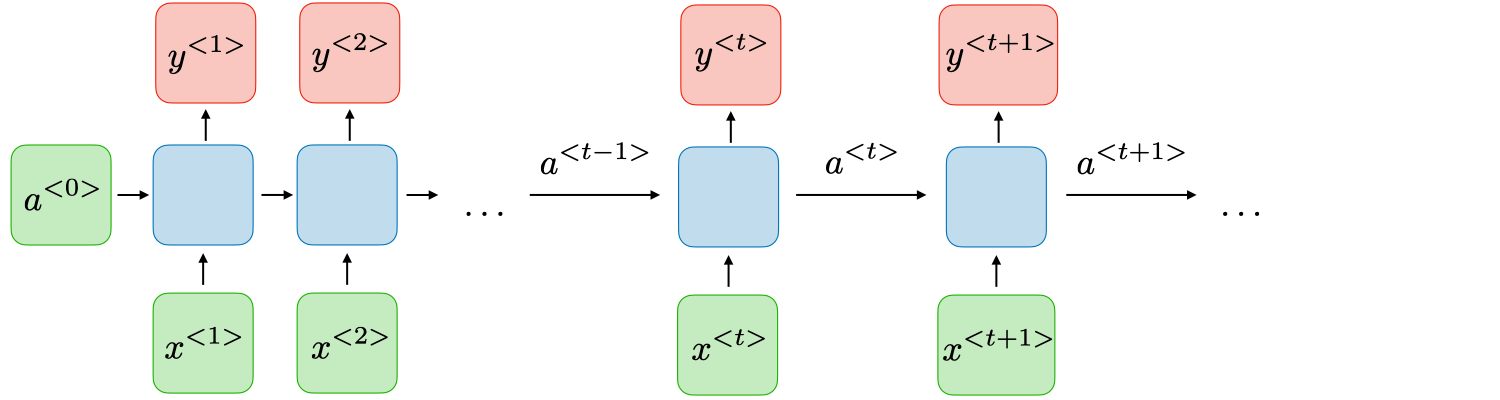
\includegraphics[scale=0.35]{figures/architecture-rnn.png}
	% To make sure citation doesn't appear in list of figures
	\caption [
	ساختار شبکه‌های عصبی بازگشتی
	]{
	ساختار شبکه‌های عصبی بازگشتی 
	\cite{rnncheat}
	}
	\label{fig:rnnarch}
\end{figure}

شبکه‌های عصبی بازگشتی
گونه‌ی خاصی از الگوریتم‌های یادگیری ماشین هستند که ساختار کلی آن‌ها در شکل
\ref{fig:rnnarch}
آمده است.
در این‌گونه شبکه‌های عصبی نیز
$x$
ها نشان‌گر داده‌های ورودی از مجموعه داده‌ها و
$y$
ها نشان‌گر خروجی‌های الگوریتم هستند.
پارامترهای تنظیم‌پذیر در واحد‌های آبی‌رنگ که به 
واحد‌های بازگشتی
\fnote{Recurrent block}
معروف هستند قرار می‌گیرند.
نکته‌ی اصلی شبکه‌های عصبی بازگشتی این است که هر واحد بازگشتی، در هنگام انجام محاسبات، از نتایج محاسبات واحد‌های محاسباتی قبل از خود استفاده می‌کند، چراکه در این صورت می‌تواند با کسب آگاهی از خروجی‌های گذشته و ترتیب آن‌ها، خروجی معنی‌داری تولید کند.
این‌گونه الگوریتم‌ها اغلب در یادگیری ویژگی‌های داده‌های ترتیبی
\fnote{Sequential data}
کاربرد دارند؛ به این معنا که نه تنها خود خروجی‌های الگوریتم، بلکه ترتیب آن‌ها هم از اهمیت بالایی برخوردار است.
نت‌های موسیقی را نیز می‌توان به صورت مجموعه‌ای از داده‌های ترتیبی در نظر گرفت، چراکه هر مجموعه‌ای از نت‌های موسیقی، صدایی آهنگین تولید نمی‌کند و ترتیب نت‌های قرار گرفته در یک ملودی نیز برای این‌که توسط گوش انسان به عنوان یک موسیقی حقیقی در نظر گرفته شوند حائز اهمیت است.

\subsubsection{حافظه‌ی طولانی کوتاه-مدت}
حافظه‌ی طولانی کوتاه-مدت
\fnote{Long short-term memory}
نوع خاصی از شبکه‌های عصبی بازگشتی است که ساختار کلی  واحد بازگشتی آن در شکل
\ref{fig:lstmblock}
آمده است.
یکی از ویژگی‌های مهمی که حافظه‌های طولانی کوتاه-مدت را در مقایسه با باقی شبکه‌های عصبی بازگشتی متمایز می‌کند، این است که به جای انتقال یک واحد اطلاعات از هر مرحله به مرحله‌ی بعدی، دو واحد اطلاعات را منتقل می‌کند.

\begin{figure}
	\centering
	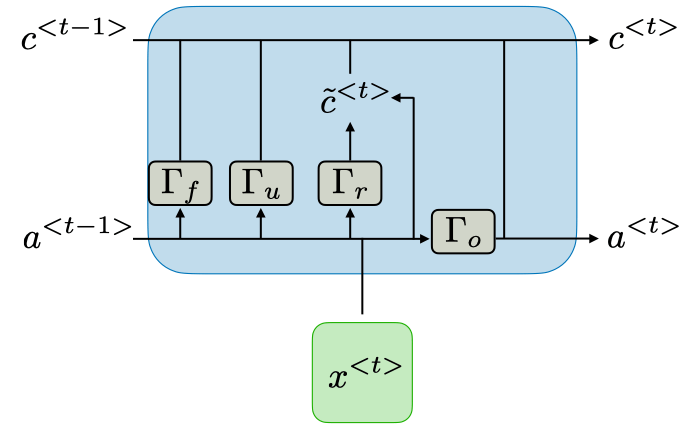
\includegraphics[scale=0.4]{figures/lstm-rec-unit.png}
	% To make sure citation doesn't appear in list of figures
	\caption [
	واحد بازگشتی حافظه‌ی طولانی کوتاه-مدت
	]{
	واحد بازگشتی حافظه‌ی طولانی کوتاه-مدت 
	\cite{rnncheat}
	}
	\label{fig:lstmblock}
\end{figure}

گیت‌های بازگشتی، واحدهای پردازشی‌ای هستند که به طور معمول در شبکه‌های عصبی بازگشتی حضور دارند و با علامت 
$\Gamma$
نشان داده می‌شوند. حالت کلی این گیت‌ها به صورت زیر است:
\begin{equation}
    \Gamma = \sigma(Wx^{(t)} + Ua^{(t-1)} + b)
\end{equation}
\myequations{گیت‌های بازگشتی}
که در معادله‌ی بالا، پارامترهای
$W, U, b \hspace{0.5mm}$
همان پارامترهای تنظیم‌پذیر الگوریتم هستند و
$\sigma$
یک تابع غیرخطی است که برای تعمیم توانایی مدل‌سازی شبکه‌های عصبی استفاده می‌شود و معمولا تابع فعال‌سازی
\fnote{Activation function}
نامیده می‌شود.
در حافظه‌های کوتاه بلند-مدت،، معمولا از تابع سیگموید
\fnote{Sigmoid function}
به عنوان تابع فعال‌سازی استفاده می‌شود که تعریف این تابع به صورت زیر است:
\begin{equation}
    S(x) = \frac{1}{1+e^{-x}} = \frac{e^x}{e^x + 1}
\end{equation}
\myequations{تابع سیگموید}

همان‌طور که در شکل
\ref{fig:lstmblock}
مشاهده می‌شود، هر واحد بازگشتی حافظه‌های طولانی کوتاه-مدت شامل چهار گیت بازگشتی است که هر کدام به منظور خاصی تعبیه شده‌اند و سعی در پیاده‌سازی رفتار خاصی را دارند.

\begin{itemize}
    \item
    گیت به‌روزرسانی
    \fnote{Update gate}
    یا 
    $\Gamma_u$
    که میزان حفظ اطلاعات مراحل گذشته در محاسبات فعلی را تعیین می‌کند.
    
    \item
    گیت ارتباط
    \fnote{Relevance gate}
    یا 
    $\Gamma_r$
    که میزان پاک‌شدن اطلاعات مراحل گذشته در محاسبات فعلی را تعیین می‌کند.
    
    \item
    گیت خروجی
    \fnote{Output gate}
    یا 
    $\Gamma_o$
    که میزان حفظ شدن اطلاعات محاسبات فعلی برای انتقال به مرحله‌ی بعدی را تعیین می‌کند.
    
    \item
    گیت فراموشی
    \fnote{Forget gate}
    یا
    $\Gamma_f$
    که میزان پاک‌شدن اطلاعات محاسبات فعلی برای انتقال به مرحله‌ی بعدی را تعیین می‌کند.
\end{itemize}

شایان ذکر است که پارامترهای این گیت‌های بازگشتی، معمولا پارامترهای مستقلی هستند و لذا به صورت جداگانه نیز بهینه‌سازی می‌شوند.

در نهایت، خروجی‌های واحد
$t$
-ام یک
حافظه‌ی کوتاه بلند-مدت که با
$c^{(t)}$
و
$a^{(t)}$
نشان داده می‌شوند،
به صورت زیر محاسبه می‌شوند:
\begin{equation}
\begin{gathered}
    \hat{c}^{(t)} = tanh(W_c[\Gamma_r * a^{(t-1)}, x^{(t)}] + b_c) \\
    c^{(t)} = \Gamma_u * \hat{c}^{(t)} + \Gamma_f * c^{(t-1)} \\
    a^{(t)} = \Gamma_o * c^{(t)}
\end{gathered}
\end{equation}
\myequations{خروجی‌های واحد بازگشتی حافظه‌ی طولانی کوتاه-مدت}

\newpage

\subsection{
شبکه‌های زایای دشمن‌گونه
\protect\fnote{Generative adversarial networks}
}
هر شبکه‌ی زایای دشمن گونه، متشکل از دو مدل یادگیری ماشین است. در هنگام مراحل یادگیری، این دو مدل با یک‌دیگر رقابت می‌کنند و سعی می‌کنند دیگری را در یک بازی مجموع-صفر
\fnote{Zero-sum game}
شکست دهند. یکی از این مدل‌ها، مدل زایا
\fnote{Generative model}
و مدل دیگر، مدل فرق‌گذار
\fnote{Discriminative model}
نام دارد. 
با فرض این‌که مجموعه داده‌ای با توزیعی
\fnote{Distribution}
مشخص موجود باشد، مدل زایا سعی می‌کند داده‌های جدیدی تولید کند که شباهت زیادی به داده‌های توزیع واقعی تولید کند. در عین حال، مدل فرق‌گذار، سعی می‌کند پس از گرفتن یک داده‌ی ورودی، تشخیص دهد که این داده متعلق به آن توزیع است یا خیر.
\\
برای واضح‌تر شدن چگونگی کارکرد شبکه‌های زایای دشمن‌گونه، می‌توان به مساله‌ی تولید پرتره اشاره کرد؛ به این معنا که مجموعه داده‌ای از عکس‌های پرتره‌ی صورت انسان‌های متفاوتی موجود است. در این حالت، مدل زایا تلاش می‌کند تا عکس پرتره‌ی جدیدی تولید کند و مدل فرق‌گذار با گرفتن ورودی‌ای، سعی می‌کند تشخیص دهد که این ورودی توسط مدل زایا تولید شده یا از مجموعه داده‌ی اصلی نمونه‌برداری شده.
در نهایت، در صورت موفق بودن تمرین این دو مدل، مدل زایا می‌تواند عکس‌های پرتره‌ی جدیدی تولید کند که کامپیوتری بودن آن‌ها حتی توسط خود انسان‌ها هم ممکن نباشد و مدل فرق‌گذار می‌تواند عکس‌های کامپیوتری را از عکس‌های واقعی به خوبی تشخیص دهد. 
% \end{equation}

\begin{figure}
	\centering
	
\includegraphics[scale=0.2]{figures/fakeperson.jpg}
	% To make sure citation doesn't appear in list of figures
	\caption [
	نمونه عکس پرتره‌ی تولید شده توسط شبکه‌ی زایای دشمن‌گونه
	]{
	نمونه عکس پرتره‌ی تولید شده توسط شبکه‌ی زایای دشمن‌گونه
	\cite{thisperson}
	}
	\label{fig:lstmblock}
\end{figure}